\documentclass[10pt,utf8]{beamer}

\mode<presentation> {
  \usetheme{Madrid}
  \setbeamercovered{transparent}
}

\usepackage{palatino}
\usepackage{graphicx}
\usepackage{array}
\usepackage{color}
\usepackage{subfigure}
\usepackage{colortbl}
\usepackage{amsmath}
\usepackage{hyperref}
\usepackage{listings}
\usepackage{fancyvrb}

\setbeamertemplate{caption}{\raggedright\insertcaption\par} %turn off caption prefix ("Figure")

\definecolor{delim}{RGB}{20,105,176}
\definecolor{numb}{RGB}{106, 109, 32}
\definecolor{string}{rgb}{0.64,0.08,0.08}

\lstdefinestyle{java}{
	basicstyle          = \normalsize\ttfamily,
	language            = java,
	numbers             = left,
	numberstyle         = \small,
	stepnumber          = 1,
	numbersep           = 5pt,
	backgroundcolor     = \color{white},
	showspaces          = false,
	showstringspaces    = false,
	showtabs            = false,
	frame               = single,
	tabsize             = 2,
	captionpos          = b,
	breaklines          = true,
	breakatwhitespace   = false,
	morestring          = [b]",
	stringstyle         = \color{blue},
	keywordstyle        = \color{magenta},
	commentstyle        = \color{gray},
	identifierstyle     = \color{black},
	moredelim           = **[is][\bfseries]{`}{`},
	moredelim           = **[is][\color{magenta}]{$}{$}, 
	fancyvrb            = true,
}


\title{Jepsen: quick intro}
\author{Vojtěch Juránek}
\institute[Red Hat]{Red Hat}
\date{May 22st 2024, Debezium F2F meeting, Brno}

\newenvironment{mylisting}
{\begin{list}{}{\setlength{\leftmargin}{1em}}\item\scriptsize\bfseries}
{\end{list}}

\newenvironment{mytinylisting}
{\begin{list}{}{\setlength{\leftmargin}{1em}}\item\tiny\bfseries}
{\end{list}}


\begin{document}

\begin{frame}
    \titlepage
\end{frame}

\begin{frame}
    \frametitle{Jepsen}
    \begin{itemize}
      \item \textit{Breaking distributed systems so you don't have to.}
      \item \textit{Jepsen is an effort to improve the safety of distributed databases, queues, consensus systems, etc.} 
    \end{itemize}
    
    \vspace{1cm}
    
    \begin{itemize}
      \item A test library written in Clojure.
      \item Makes easy to setup and test distributed system in a test.
      \item Developed by \color{blue}\href{https://aphyr.com/about}{Kyle Kingsbury}\color{black}, a.k.a "Aphyr".
    \end{itemize}
\end{frame}

\begin{frame}
    \frametitle{Jepsen architecture}
    \begin{figure}
        \centering
        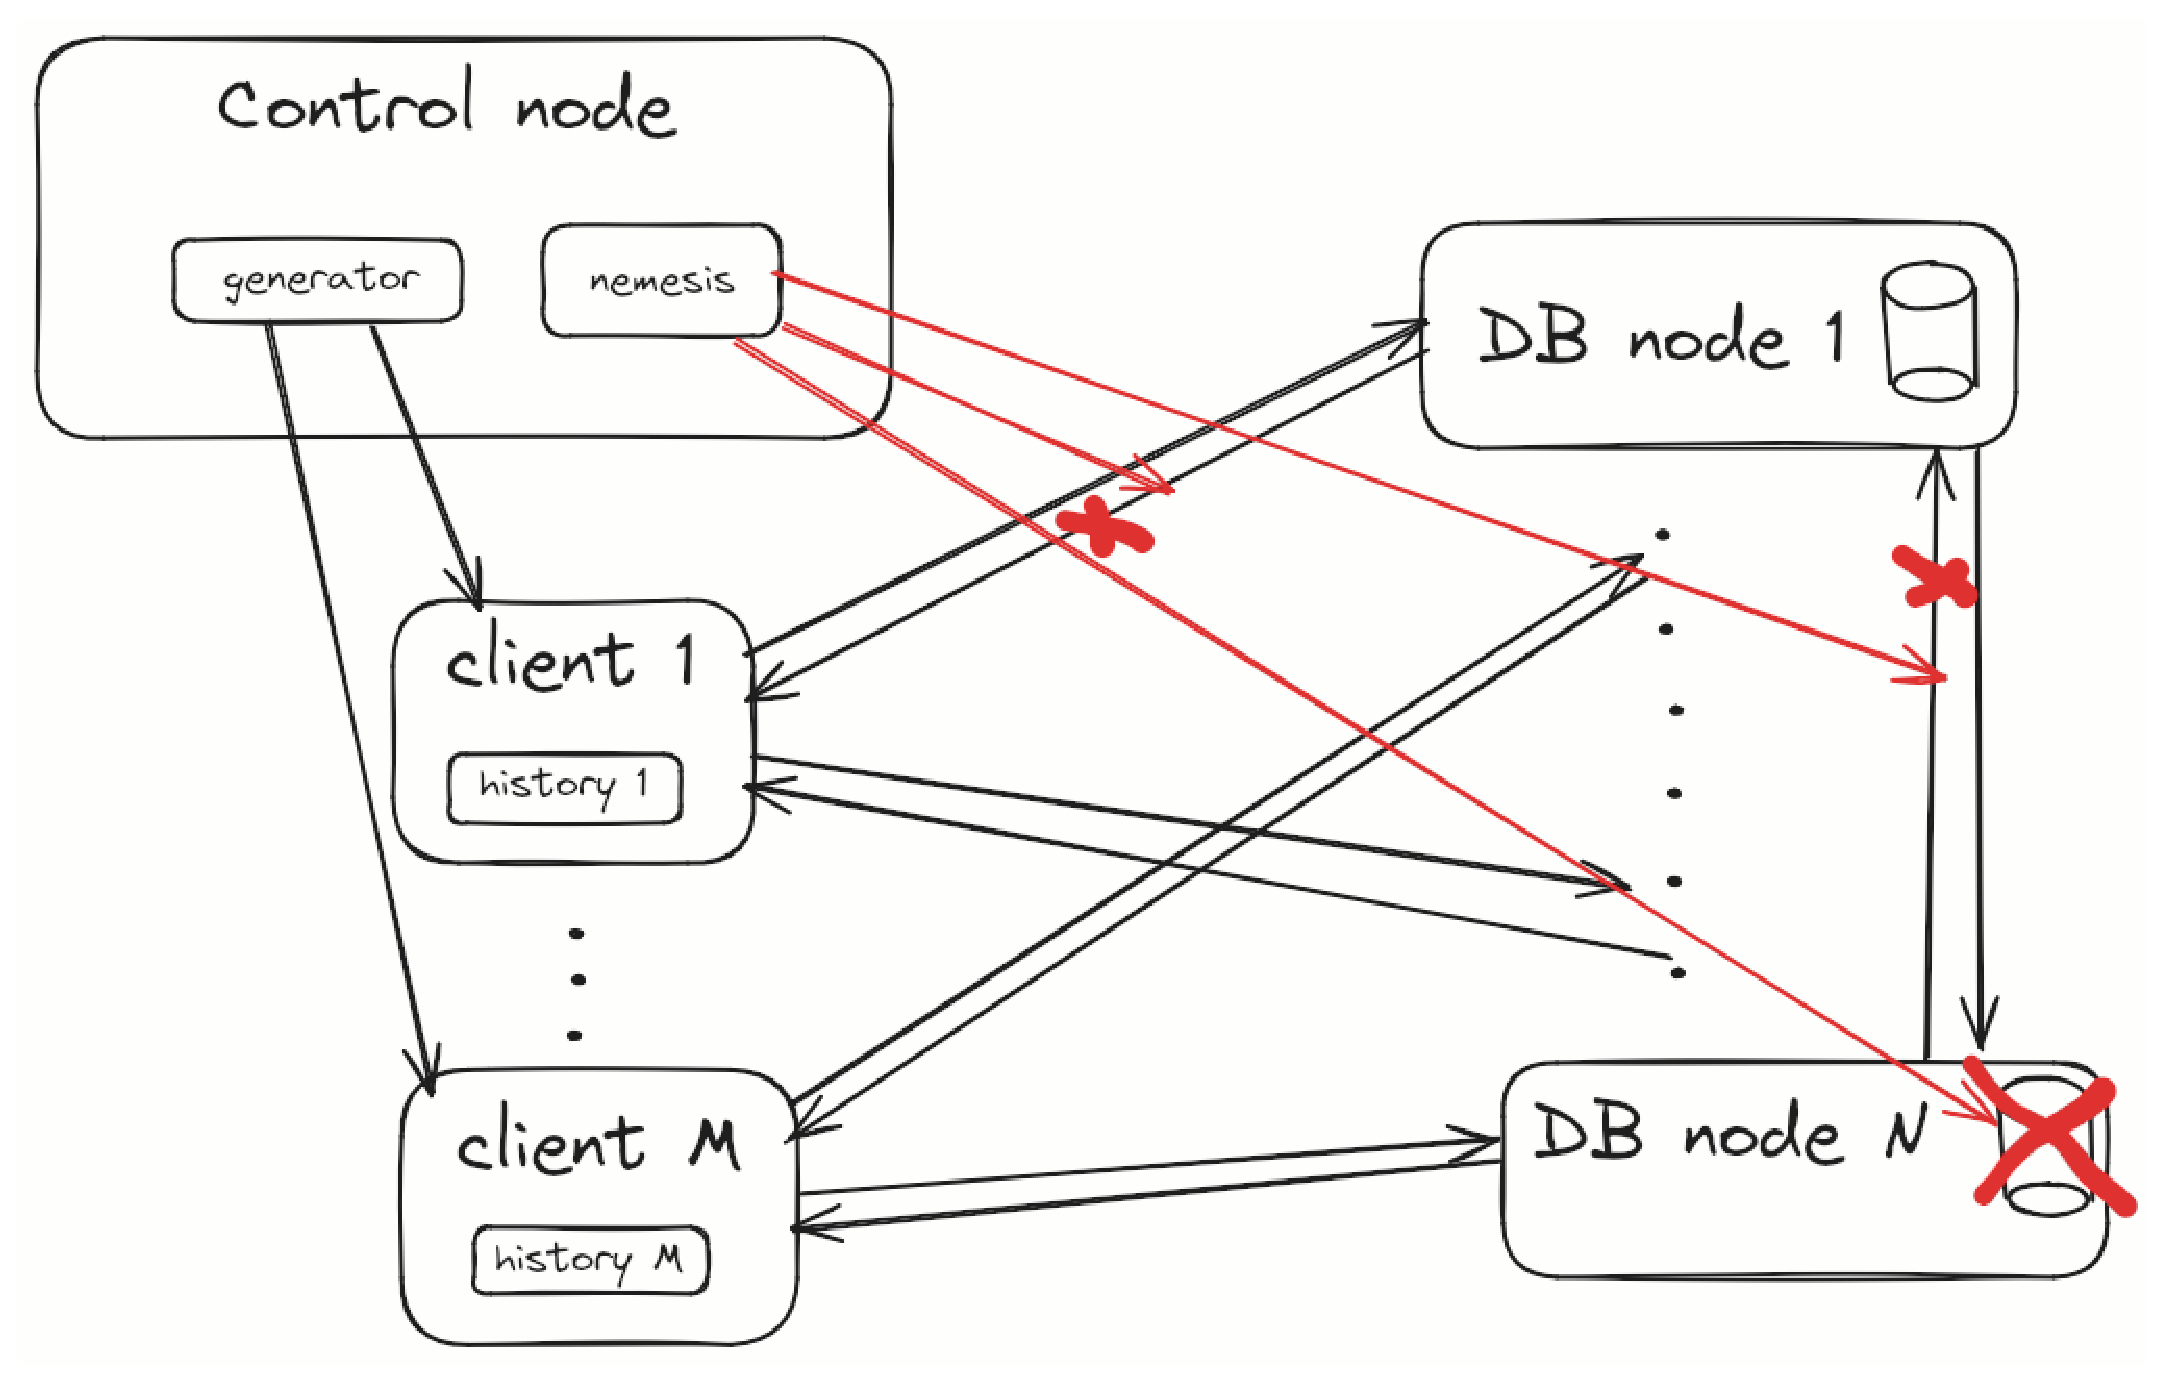
\includegraphics[height=6cm]{./img/jepsen_nodes.eps}
    \end{figure}
    \begin{itemize}
      \item Transaction histories are analyzed by the checker once the test finishes. \\
      \item Main work of the checker is done by Elle.
    \end{itemize}
\end{frame}

\begin{frame}
    \frametitle{Elle}
    \begin{itemize}
      \item \color{blue}\href{https://github.com/jepsen-io/elle}{Elle}\color{black}~is a transaction consistency checker.
      \item Search for cycled in transaction dependencies graph.
    \end{itemize}
    \begin{figure}
        \centering
        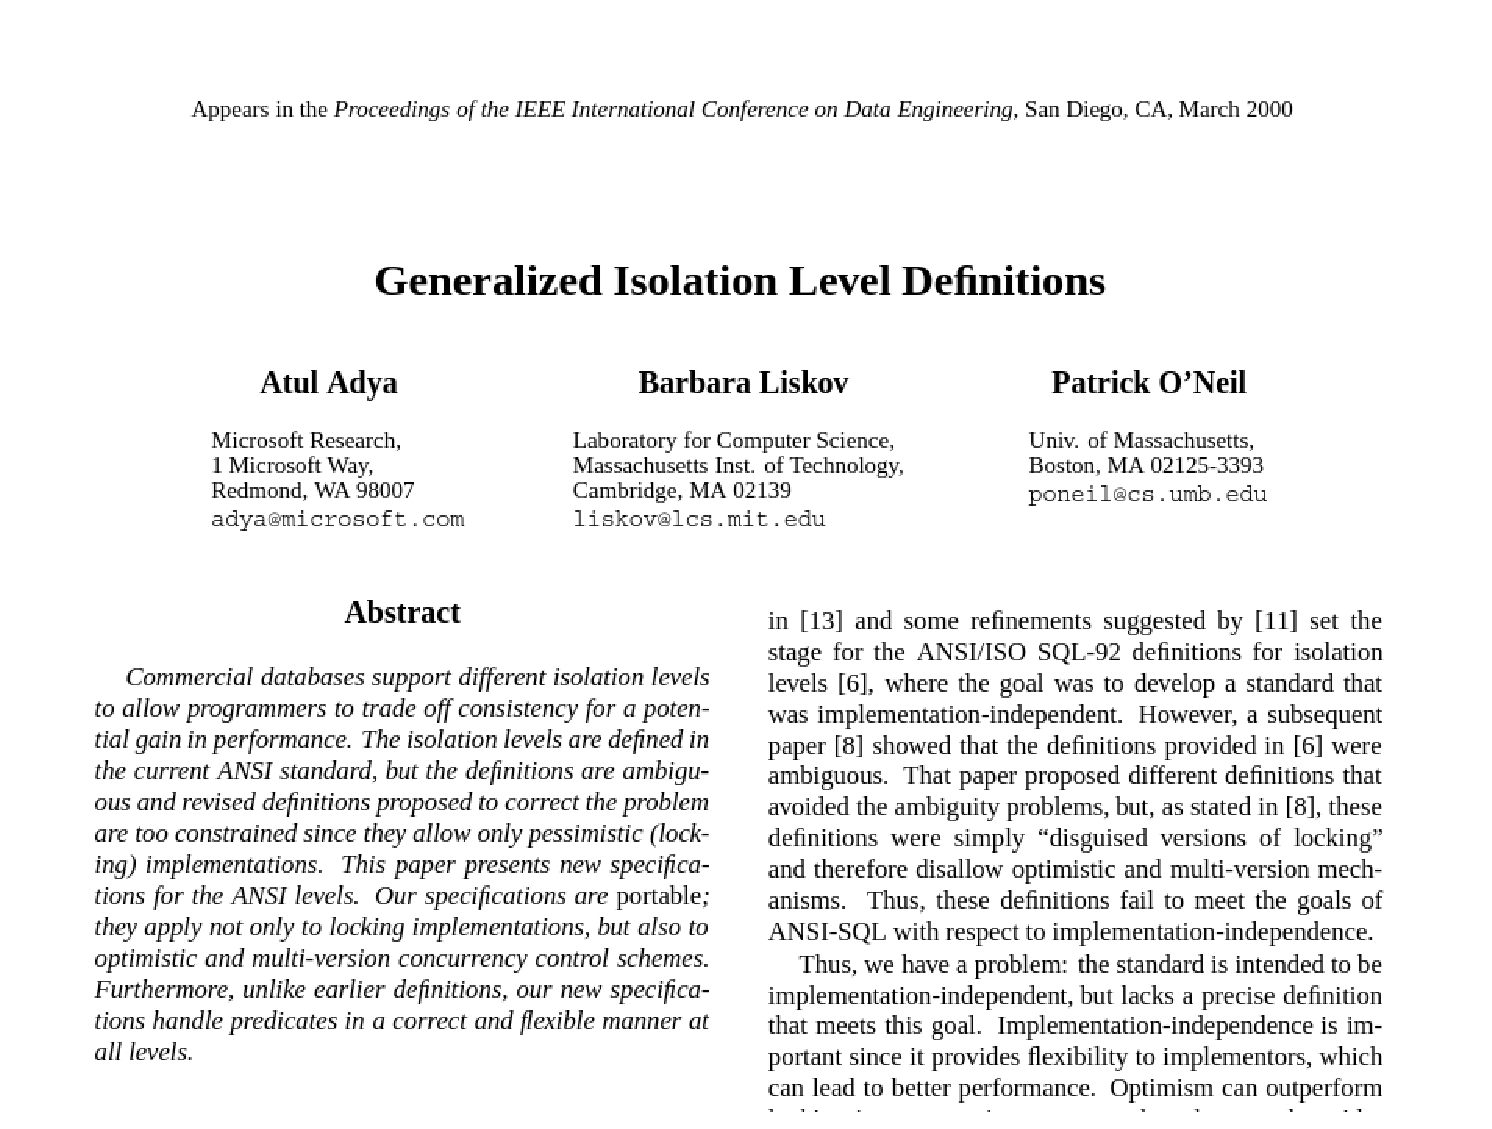
\includegraphics[height=6cm]{./img/adya_paper.eps}
    \end{figure}
\end{frame}

\begin{frame}
    \frametitle{Example: Postgres G2-item}
    \begin{itemize}
      \item G2-item in Postgres, violates repeatable-read isolation level.
      \item See \color{blue}\href{https://jepsen.io/analyses/postgresql-12.3}{PostgreSQL 12.3 jepsen report}\color{black}~and \color{blue}\href{https://github.com/ept/hermitage/blob/master/postgres.md\#write-skew-g2-item}{Kleppmann's Hermitage: Testing transaction isolation levels}\color{black}
    \end{itemize}
    \begin{figure}
        \centering
        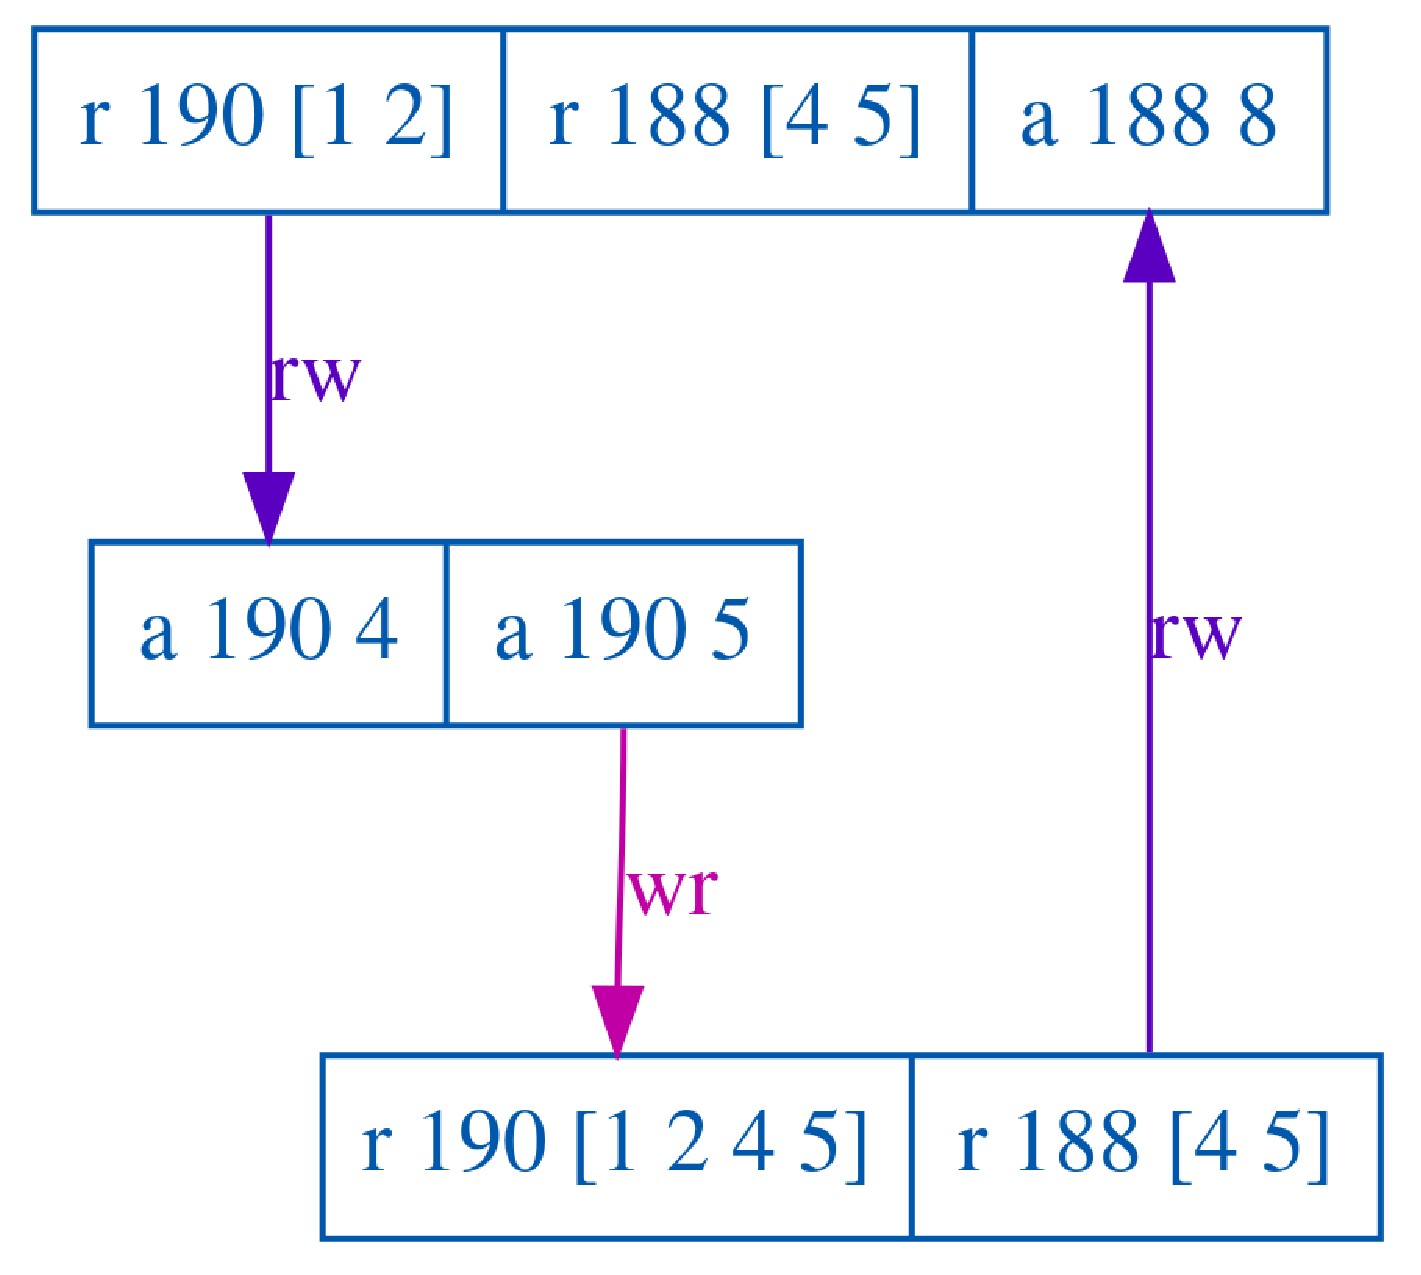
\includegraphics[height=5cm]{./img/postgres_g2.eps}
         \caption{\tiny{Source: \url{https://jepsen.io/analyses/postgresql-12.3}}}
    \end{figure}
\end{frame}

\begin{frame}
    \frametitle{Practical}
    \begin{itemize}
      \item Jepsen is supported on Linux bare metal, VMs and LXC.
      \item Docker is available, but not supported.
      \item Available very good \color{blue}\href{https://github.com/jepsen-io/jepsen/blob/main/doc/tutorial/index.md}{tutorial}\color{black}.
      \item Clojure makes the development harder, but the actual hard thing is to nail down the right testing scenarios which reveal the issues.
    \end{itemize}
\end{frame}

\begin{frame}
    \frametitle{Jepsen tests for Debezium}
    \begin{itemize}
      \item Could find issues like recent \color{blue}\href{https://issues.redhat.com/browse/DBZ-7816}{DBZ-7816}\color{black}.
      \item There are tests for \color{blue}\href{https://github.com/jepsen-io/postgres}{Postgres}\color{black}~and \color{blue}\href{https://github.com/jepsen-io/mysql}{MySQL}\color{black} - we should be able to reuse at least some parts of the code.
    \end{itemize}
\end{frame}

\begin{frame}
    \frametitle{Resources}
    \begin{itemize}
        \color{blue}
        \item \href{https://jepsen.io/}{https://jepsen.io/}
        \item \href{https://www.youtube.com/watch?v=OPJ_IcdSqig}{Black-box Isolation Checking with Elle}
        \item \href{https://github.com/ept/hermitage/}{Hermitage: Testing transaction isolation levels}
        \item \href{https://github.com/jepsen-io/maelstrom}{Maelstrom}\color{black}~a workbench for learning distributed systems by writing your own
    \end{itemize}
\end{frame}

\begin{frame}
    \frametitle{Questions?}
    \centering
     \textbf{\Huge{Thank you!}}
    
    \vspace{1.5cm}
    
    \textbf{\Huge{Questions?}}
    
    \vspace{1cm}
\end{frame}

%%%%%%%%%%%%%%%%%%%%%%%%%%%%%%%%%%%%%%%%%%%%%%%%%%%%%%%%%%%%%%%%%%%%%%%%%%%%%%%%%%%%%%%%%%%%%%%%%
%%% BACKUP
%%%%%%%%%%%%%%%%%%%%%%%%%%%%%%%%%%%%%%%%%%%%%%%%%%%%%%%%%%%%%%%%%%%%%%%%%%%%%%%%%%%%%%%%%%%%%%%%%

% \begin{frame}
%     \centering
%     \huge{\textbf{Backup slides}}
% \end{frame}

\end{document}
